%%
%% This is file `sample-sigconf.tex',
%% generated with the docstrip utility.
%%
%% The original source files were:
%%
%% samples.dtx  (with options: `sigconf')
%%
%% IMPORTANT NOTICE:
%%
%% For the copyright see the source file.
%%
%% Any modified versions of this file must be renamed
%% with new filenames distinct from sample-sigconf.tex.
%%
%% For distribution of the original source see the terms
%% for copying and modification in the file samples.dtx.
%%
%% This generated file may be distributed as long as the
%% original source files, as listed above, are part of the
%% same distribution. (The sources need not necessarily be
%% in the same archive or directory.)
%%
%% The first command in your LaTeX source must be the \documentclass command.
\documentclass[conference]{IEEEtran}

\usepackage[utf8]{inputenc}
\usepackage{multirow}
\usepackage[inline]{enumitem}
\usepackage{xcolor}
\usepackage{booktabs}
\usepackage{hyperref}
\usepackage{amsmath}
\usepackage{amssymb}
\usepackage{graphicx}
\usepackage[numbers]{natbib}
\usepackage{subfig}

\usepackage[nomain, toc, acronym]{glossaries}
\glsdisablehyper

\newcommand\note[2]{{\color{#1}#2}}
\newcommand\todo[1]{{\note{red}{TODO: #1}}}

%%
%% end of the preamble, start of the body of the document source.
\begin{document}

%%
%% The "title" command has an optional parameter,
%% allowing the author to define a "short title" to be used in page headers.
\title{An in-depth study of Explainability and Adversarial Robustness for RNNs}

\author{\IEEEauthorblockN{Alexander Hartl,
Maximilian Bachl, Joachim Fabini, Tanja Zseby}
\IEEEauthorblockA{Technische Universität Wien\\
firstname.lastname@tuwien.ac.at}}

%\date{\today}

% \IEEEoverridecommandlockouts
% \IEEEpubid{\begin{minipage}[t]{\textwidth}\ \\[10pt]
%         \centering\normalsize{xxx-x-xxxx-xxxx-x/xx/\$31.00 \copyright 2018 IEEE}
% \end{minipage}}

% \renewcommand*{\bibfont}{\footnotesize}

\maketitle%

\thispagestyle{plain}
\pagestyle{plain}

\newacronym{ml}{ML}{Machine Learning}
\newacronym{dl}{DL}{Deep Learning}
\newacronym{aml}{AML}{Adversarial Machine Learning}
\newacronym{ids}{IDS}{Intrusion Detection System}
\newacronym{rnn}{RNN}{Recurrent Neural Network}
\newacronym{fgsm}{FGSM}{Fast Gradient Sign Method}
\newacronym{cw}{CW}{Carlini-Wagner method}
\newacronym{pgd}{PGD}{Projected Gradient Descent}
\newacronym{pdp}{PDP}{Partial Dependence Plot}
\newacronym{ars}{ARS}{Adversarial Robustness Score}
\newacronym{ttl}{TTL}{Time-to-Live}
\newacronym{dos}{DoS}{Denial-of-Service}
\newacronym{iat}{IAT}{Interarrival time}
\newacronym{tcp}{TCP}{Transmission control protocol}

\begin{abstract}

\glspl{rnn} yield attractive properties for performing intrusion detection on network data.
However, with the rise of ubiquitous \gls{ml} systems, malicious actors have been catching up quickly to find new ways to exploit \gls{ml} for profit. Recently developed \gls{aml} techniques focus on computer vision and their applicability to network traffic is not straightforward: Network packets expose fewer features than an image, are sequential and impose several constraints on their features. For example, destination ports cannot be modified since that could impair communication.

We show that despite these completely different characteristics, adversarial samples can be reliably generated for \glspl{rnn}.
Since traditional evaluation metrics such as accuracy are not sufficient for quantifying the adversarial threat, we propose the \gls{ars}. %as a countermeasure. % AH. the score alone is not yet a countermeasure 
To understand a classifier's potential for misclassification, we extend existing explainability techniques and propose new ones, particularly suitable % specifically crafted %AH most can also be used for non-sequential models, so lets not restrict applicability too much
for sequential data. Applying them shows that already the first packets of a communication flow are of crucial importance and are likely going to be targeted by attackers. Feature importance methods show that even relatively unimportant features can be effectively abused to generate adversarial samples.
As a countermeasure, we develop an easy-to-use adversarial training procedure %and can confirm that it
which significantly and successfully reduces the attack surface and improves \gls{ars}.

\end{abstract}

%%
%% The abstract is a short summary of the work to be presented in the
%% article.
%\begin{abstract}
%  A clear and well-documented \LaTeX\ document is presented as an
%  article formatted for publication by ACM in a conference proceedings
%  or journal publication. Based on the ``acmart'' document class, this
%  article presents and explains many of the common variations, as well
%  as many of the formatting elements an author may use in the
%  preparation of the documentation of their work.
%\end{abstract}

\maketitle

\section{Introduction}

There is a significant body of scientific work focusing on the detection of unwanted behavior in networks. In the past, a viable way of performing intrusion detection was to inspect the content of packets themselves and detect if a packet delivers potentially harmful content. More recently, with the rise of omnipresent encryption, available features have changed. Since payload is no longer avilable, the focus now lies on features that are always available to network monitoring equipment such as port numbers, protocol flags, packet size etc. 

Network communication is usually grouped into \textit{flows}, which are commonly defined as a sequence of packets sharing certain properties, between two applications that may be located at different physical locations.
When analyzing flows, not only the aforementioned features are available but also features related to the timing of the individual packets. % as well as their size. %AH: don't see why pkt size is not available without flows
For example, a specific attack might require the attacker to send three small packets and the victim to reply with two large packets followed by a small one to the attacker. Various approaches have been proposed to extract features from flows and then perform anomaly detection with the extracted flows \cite{meghdouri_analysis_2018}.
While these approaches frequently work well, it is problematic that the whole flow has to be received first and only afterwards an anomaly can be detected. Thus, we design a network \gls{ids} that operates on a per-packet basis and decides if a packet is anomalous based on features that are available even for traffic that is encrypted above the transport layer, like for example TLS or QUIC.
At the same time, an \gls{rnn}-based \gls{ids} has the benefit of avoiding tedious feature selection procedures while providing any available information to the classifier.
We show that our system has similar performance to other flow-based anomaly detection systems but can commonly detect anomalies \textit{before} the flow is over. 

With the recent rise of interest in \gls{aml} techniques, also \gls{aml} for \glspl{ids} has been investigated. For example, \cite{bachl_walling_2019} investigates remedies for poisoning attacks on \glspl{ids}.
In this research, we investigate whether adversarial samples can be found for our \gls{rnn}-based model. This is not a trivially answerable question since adversarial samples have mostly been analyzed in the context of computer vision. Our scenario significantly deviates from this in several ways because \begin{enumerate*}
\item the number of features is significantly smaller and
\item only certain features can be manipulated by an adversary (for example the destination port cannot be manipulated)
\end{enumerate*}.

Surprisingly, we can confirm that adversarial samples can be found even when considering these tight constraints. % mentioned before.
Thus, we argue that traditional methods like, e.g., accuracy are not sufficient for evaluating security-sensitive \gls{ml} systems.
We propose the \acrfull{ars} as a new performance score, which precisely captures the notion of how easily an adversary can generate adversarial samples. 

In practice, a further crucial requirement for \gls{ml}-based \glspl{ids} 
is that the classifiers decisions can be interpreted, recently giving rise to increasing interest in explainability methods. Also in this case, common methods are designed to work with images or tabular data but not with sequences. Hence, we extend existing explainability methods such as \glspl{pdp} \cite{friedman_greedy_2001} for sequential data. These show the varying characteristics of different attacks and they aid with visualizing potentially vulnerable features for adversaries.
Astonishingly, feature importance methods reveal that the manipulable features, that are left for modification by adversaries are not even particularly significant for the classification outcome. %Especially the first packets of a flow are critical for determining the decision of a recurrent \gls{ids}. 

%Since common explainability methods are designed to work with images or tabular data but not sequences, we extend existing explainability methods such as \glspl{pdp} \cite{friedman_greedy_2001} for sequential data. These show the varying characteristics of different attacks and they aid with visualizing potentially vulnerable features for adversaries.

Based on the insights gained by the feature importance and explainability methods, we propose two defence methods.
%develop a simple method for defending against adversaries who can manipulate arbitrary packets by simply leaving out potentially manipulable information from the classification process.
On the one hand, by simply leaving out manipulable features, we obtain a classifier which is slightly less accurate but is still useful to be deployed in a real scenario. Furthermore, we develop a custom adversarial training procedure which especially focuses on ease of use and low resource consumption and aims to keep the number of additionally introduced training hyperparameters low. With this novel strategy we can reduce the attack surface and harden the resulting \gls{ids} while retaining similar classification performance. % like for the original \gls{ml} model. 

\section{An \gls{rnn}-based classifier}

% \begin{table}[b]
% \caption{occurrence frequency of attack types.} \label{tab:occurrence}
% \centering
% \begin{tabular}{l r} \toprule
% Attack type & Proportion \\
% \midrule
% Normal                                                         & $0.747468$ \\
% DoS / DDoS:DoS Hulk                                            & $0.101014$ \\
% PortScan:PortScan - Firewall off                               & $0.069020$ \\
% DDoS:LOIT                                                      & $0.040784$ \\
% Infiltration:Dropbox download                                  & $0.032982$ \\
% DoS / DDoS:DoS GoldenEye                                       & $0.003224$ \\
% DoS / DDoS:DoS Slowhttptest                                    & $0.001819$ \\
% DoS / DDoS:DoS slowloris                                       & $0.001680$ \\
% Brute Force:SSH-Patator                                        & $0.001107$ \\
% Botnet:ARES                                                    & $0.000327$ \\
% Web Attack:XSS                                                 & $0.000293$ \\
% PortScan:PortScan - Firewall on                                & $0.000165$ \\
% Brute Force:FTP-Patator                                        & $0.000110$ \\
% Web Attack:Sql Injection                                       & $0.000006$ \\
% DoS / DDoS:Heartbleed                                          & $0.000001$ \\
% \bottomrule
% \end{tabular}
% \label{tab:occurrence}
% \end{table}

\begin{table}[b]
\caption{Occurrence frequency of attack types.}
\label{tab:occurrence}
\centering
\subfloat[CIC-IDS-2017\label{fig:cicids17proportions}
]{
\begin{tabular}{l r}
\toprule
Attack type & \hspace*{-4mm}Proportion \\ \midrule
DoS Hulk	&	10.10\%	\\
PortScan, Firewall	&	6.90\%	\\
DDoS LOIT	&	4.08\%	\\
Infiltration	&	3.30\%	\\
DoS GoldenEye	&	0.32\%	\\
DoS SlowHTTPTest	&	0.18\%	\\
DoS Slowloris	&	0.17\%	\\
Brute-force SSH	&	0.11\%	\\
Botnet ARES	&	0.03\%	\\
XSS attack	&	0.03\%	\\
PortScan, no Fw.	&	0.02\%	\\
Brute-force FTP	&	0.01\%	\\
SQL injection	&	$<$0.01\%	\\
Heartbleed	&	$<$0.01\%	\\
\bottomrule
\end{tabular}
}{}
\subfloat[UNSW-NB15\label{fig:unswnb15proportions}
]{
\begin{tabular}{l r}
\toprule
Attack type & \hspace*{-4mm}Proportion \\ \midrule
Exploits	&	1.42\%	\\
Fuzzers	&	1.01\%	\\
Reconnaissance	&	0.58\%	\\
Generic	&	0.21\%	\\
DoS	&	0.19\%	\\
Shellcode	&	0.08\%	\\
Analysis	&	0.03\%	\\
Backdoors	&	0.02\%	\\
Worms	&	0.01\%	\\
\bottomrule
\end{tabular}
}{}
\end{table}

We implemented a three-layer LSTM-based classifier with 512 neurons at each layer. As the input features we use 
source port, destination port, protocol identifier, packet length, \gls{iat} to the previous packet in the flow, packet direction (if packet goes there or back) and all \gls{tcp} flags (0 if the flow is not \gls{tcp}).
% \begin{itemize*}
% \item source port
% \item destination port
% \item protocol identifier
% \item packet sizes
% \item \glspl{iat} of packets
% \item packet directions (if packet goes there or back)
% \item all \gls{tcp} flags (0 if the flow is not \gls{tcp})
% \end{itemize*}.
We omitted \gls{ttl} values, as they are likely to lead to unwanted prediction behaviour \cite{bachl_walling_2019}.  Among the used features, source port, destination port and protocol identifier are constant over the whole flow while the others vary.
We use Z-score normalization and a train/test split of 2:1.

For evaluation, we use the \textit{CIC-IDS-2017} \cite{sharafaldin_toward_2018} and \textit{UNSW-NB15} \cite{moustafa_unsw-nb15:_2015} datasets which each include more than 2 million flows of network data, containing both benign traffic and a large number of different attacks. Attacks contained in the datasets are shown in \autoref{tab:occurrence}.
\autoref{tab:performance_results} shows that our classifiers achieve an accuracy that is similar to previous work based on these datasets~\cite{meghdouri_analysis_2018,bachl_walling_2019}. However, unlike these classifiers, our recurrent classifier has the advantage of being able to detect attacks already before they are over.

\begin{table}
% Evaluated using
% ./python learn.py --dataroot flows.pickle --net runs/Oct26_00-03-50_gpu/lstm_module_1284.pth --function test --batchSize 512
% ./python learn.py --dataroot flows15.pickle --net runs/Oct28_15-41-46_gpu/lstm_module_997.pth --function test --batchSize 512
% on Dec. 4th
\caption{Detection performance on a packet and flow level.} \label{tab:performance_results}
\centering
\begin{tabular}{l r r r r} \toprule
& \multicolumn{2}{c}{CIC-IDS-2017} & \multicolumn{2}{c}{UNSW-NB15} \\
	&	Packet	&	Flow	&	Packet	&	Flow	\\	\midrule
Accuracy	&	0.991	&	0.997	&	0.995	&	0.983	\\	
Precision	&	0.970	&	0.997	&	0.834	&	0.786	\\	
Recall	&	0.978	&	0.991	&	0.876	&	0.726	\\	
F1	&	0.974	&	0.994	&	0.855	&	0.755	\\	
Youden	&	0.972	&	0.990	&	0.873	&	0.719	\\	


\bottomrule
\end{tabular}
\end{table}

\section{Adversarial attacks}
\label{sec:adv}
We now investigate whether known \gls{aml} methods can be used for generating adversarial flows, i.e. minimally different attack flows which are classified as benign, for our \gls{rnn}.
% In our scenario, most features such as, e.g., \gls{tcp} flags cannot be easily manipulated because their manipulation might violate the \gls{tcp} and thus cause communication to fail.
% Hence, we experiment whether by manipulating the \glspl{iat} and packet lengths of the first packets, the classifier might be fooled.
% Our scenario is quite different from how generating adversarial samples usually works: We have significantly less features than in, for example, an image. Furthermore, only two out of those few features can be manipulated. And even these features cannot be manipulated freely: Besides the constraints that packet size and \gls{iat} cannot become negative there are also more problem-specific constraints:

A network packet contains significantly less features than, e.g., an image and, furthermore, most features such as \gls{tcp} flags cannot be easily manipulated, as their manipulation might violate the protocol specifications and thus cause communication to fail. We identify the packet length and the \gls{iat} as features which are most likely to be exploited, but even these features cannot be manipulated freely. Beside the non-negativity constraint,  there are also more problem-specific constraints:
\begin{itemize}[topsep=0pt,wide,labelwidth=!,labelindent=0pt]
\item Only packets can be manipulated which are transmitted by the attacker.
Except for botnet and backdoor traffic, which is entirely controlled by an attacker, thus only packets travelling in one direction can be manipulated.
 %This means the attacker can only control one direction (except for botnets where both sides are attackers).
\item Packets must not be smaller than initially, as otherwise less information could be transmitted or packets might be rendered syntactically invalid.
\item \glspl{iat} must not decrease, as otherwise the physical speed of data transmission can be violated in some cases. An in-depth analysis of when the reduction of \glspl{iat} is possible, would come with substantial effort, so we generally disallowed it. %a reduction of this feature.
\end{itemize}

Several \gls{aml} methods have been proposed in the recent literature, achieving different speed-quality tradeoffs: 
\cite{szegedy_intriguing_2014} shows that it is possible to create adversarial samples for an image, which look similar to the original image but are classified wrongly. \cite{goodfellow_explaining_2015} develops the \gls{fgsm}, which makes easy generation of adversarial samples possible. \cite{papernot_crafting_2016} explores the use of \gls{aml} for \glspl{rnn}, but lacks import \gls{aml} methods, which we consider in this paper.

As finding adversarial flows is particularly difficult in our case, % for the reasons we discussed above,
we preferred methods  producing high-quality adversarial samples while not being as fast as other methods. We implemented the following \gls{aml} methods.

\subsection{Carlini-Wagner}
We implemented the \gls{cw} \cite{carlini_towards_2017}, which performs gradient descent on the optimization objective
\begin{equation} \label{eq:carliniWagner}
d(X,\tilde X) + \epsilon  \max(Z(\tilde X), 0).
\end{equation}
Here, $d(\cdot)$ is a distance metric and $\epsilon \in \mathbb R^+$ is a parameter governing the tradeoff achieved between attack success and distance from the original flow. Furthermore, $Z(\cdot)$ denotes the neural network's logit output, $X$ denotes the original flow and $\tilde X$ the adversarial flow under optimization.

We used $\ell_1$ norm as distance metric and \gls{pgd} for meeting the real-world constraints discussed above.

The method minimizes the adversarial sample's distance so that the network's decision is just between attack and normal traffic. In the present context, we need to make sure that the classifier's prediction would actually be normal traffic, even though a certain level of noise will be added to \glspl{iat} due to the network between attacker and victim. Instead of the above equation \ref{eq:carliniWagner} we therefore used the optimization objective
\begin{equation}
d(X,\tilde X) + \epsilon  \max(Z(\tilde X), -0.2),
\end{equation}
i.e. we require a slight level of confidence that our adversarial samples are not classified as attack traffic. A logit value of $-0.2$ corresponds to a confidence of 55\% for the sample to be benign.

\subsection{$\ell_\infty$-bounded Projected Gradient Descent}
\cite{madry_towards_2018} uses a method for generating adversarial samples which deploys \gls{pgd}  to minimize the network's negative loss function while constraining the achieved $\ell_\infty$ distance from the original samples.

\subsection{Fast Gradient Sign Method}
Finally, we also tested the Fast Gradient Sign Method (FGSM), which was initially proposed in \cite{goodfellow_explaining_2015} and perhaps is the most frequently used method for generating adversarial samples. FGSM can be considered a single pass of \gls{pgd} on the loss function with an equality constraint on the $\ell_\infty$ distance, i.e. the adversarial sample is found as
\begin{equation}
\tilde X = X + \epsilon \text{sgn}( \nabla_X L(X)),
\end{equation}
where $L(X)$ denotes the network's loss function and $\epsilon$ denotes the achieved $\ell_\infty$ distance.


\begin{figure}[t]
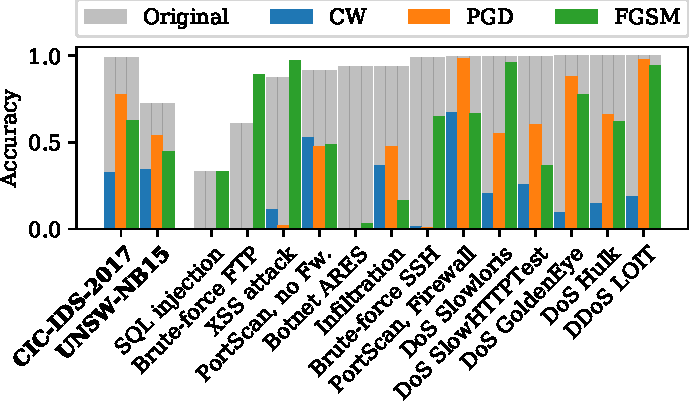
\includegraphics[width=\columnwidth]{../plots/adv_comparison/adv_comparison_17.pdf}
\caption{Attack success ratios for both dataset and per attack family for CIC-IDS-2017. Depicted are flow detection accuracies for adversarial flows and for unmodified flows.}
\label{fig:adv_per_family}
\end{figure}


\subsection{Evaluation}
\autoref{fig:adv_per_family} depicts the performance for the investigated algorithms for both datasets and for each attack family in CIC-IDS-2017. 
We used \gls{cw} with a tradeoff of 1 and, to provide a fair comparison, for \gls{fgsm} and \gls{pgd} we used an average $\ell_\infty$ distance as observed for \gls{cw}.

As expected, \gls{cw}  delivers the best performance and FGSM, while being the fastest of all investigated algorithms, delivers the worst performance.
%\autoref{fig:adv_per_family} depicts how successful the attack is for individual attack families.
The figure shows significant differences for detecting different attack families in the first place. However, also for generating adversarial flows some attack families are more susceptible than others. However, the results match to a high degree with our expectations. For example, SQL injection attacks apparently are closer to normal traffic than \gls{dos} attacks and, hence, finding adversarial samples should be easier.


It is interesting to note that increasing the $\ell_\infty$ bound for \gls{pgd} did not yield significantly improved performance. We can thus confirm the recommendation by \cite{carlini_towards_2017} to perform gradient descent on the logit output instead of the loss for good results.

\autoref{fig:adv_cw} depicts the success ratio and average distance for \gls{cw} for different tradeoffs $\epsilon$.
%\autoref{fig:adv_cw} depicts the ratio of attack flows which were successfully misclassified as benign with respect to the final packet along with the resulting distance from the original sample.
Evidently, the larger the tradeoff $\epsilon$, the better the attack works, but also distances from original flows become higher.
Hence, with acceptable distance values we were able to generate adversarial samples for about 80\% of attack samples.
The figure suggests that a tradeoff value between 0.5 and 1 would be ideal to find adversarial samples with a low enough distance from real samples.
This conclusion might be misleading, however, as due to the objective function \eqref{eq:carliniWagner} the distance cannot become larger anymore for one sample as soon as an adversarial sample has been found. %, when performing optimization as depicted by the objective function .
Hence, the depicted distance increase presumably is due to samples for which no adversarial sample could be found for lower $\epsilon$ values.




\begin{figure}[b]
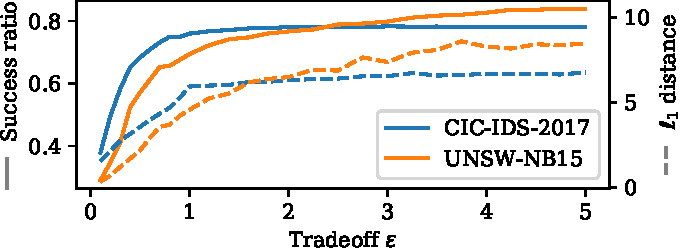
\includegraphics[width=\columnwidth]{../plots/adv_comparison/tradeoff.pdf}
% 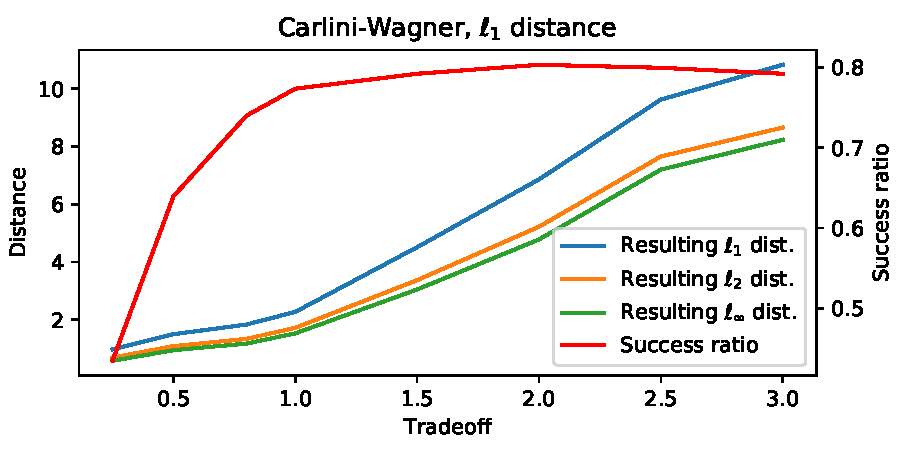
\includegraphics[width=0.49\textwidth]{adv_plots/cwl1.pdf}
% 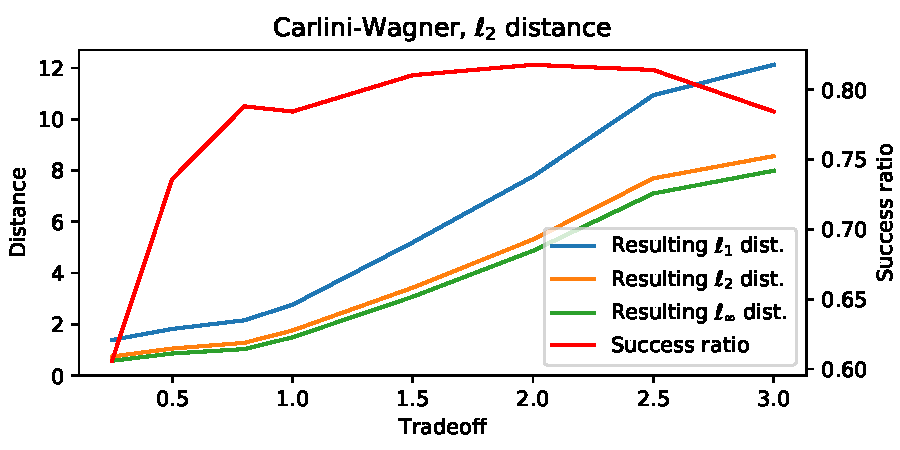
\includegraphics[width=0.49\textwidth]{adv_plots/cwl2.pdf}
\caption{Performance of \gls{cw} with different $\epsilon$ values.}
\todo{I guess the irregularity at eps=1 hints at too few iterations. Currently rerunning with 1000 base iterations}
\label{fig:adv_cw}
\end{figure}

% \begin{table*}
% \caption{Attack success ratios per attack family. Depicted are flow detection accuracies for adversarial flows (left numbers) and flow detection accuracies for unmodified flows (right numbers).}
% \label{tab:adv_per_family}
% \centering
% \begin{tabular}{llllllllll}
% \toprule
% Attack type & \multicolumn{2}{l}{FGSM} & \multicolumn{2}{l}{Carlini-Wagner, $\ell_1$} & \multicolumn{2}{l}{Carlini-Wagner, $\ell_2$} & \multicolumn{2}{l}{$\ell_\infty$-bounded \gls{pgd}} \\
% \cmidrule(r){2-3} \cmidrule(lr){4-5} \cmidrule(l){6-7} \cmidrule(l){8-9}
% & adv. & orig. & adv. & orig. & adv. & orig. & adv. & orig. \\
% \midrule
% Botnet:ARES	&	0.0000 & 0.0000	&	0.0000 & 0.0000	&	0.0000 & 0.0000	&	0.0000 & 0.0000	\\
% Brute Force:FTP-Patator	&	0.2800 & 0.5800	&	0.1600 & 0.5800	&	0.1600 & 0.5800	&	0.2800 & 0.5800	\\
% Brute Force:SSH-Patator	&	0.8300 & 1.0000	&	0.0000 & 1.0000	&	0.0000 & 1.0000	&	0.8900 & 1.0000	\\
% DDoS:LOIT	&	0.8300 & 0.8600	&	0.6400 & 0.8600	&	0.5600 & 0.8600	&	0.8200 & 0.8600	\\
% DoS / DDoS:DoS GoldenEye	&	0.8900 & 1.0000	&	0.5000 & 1.0000	&	0.4200 & 1.0000	&	0.9200 & 1.0000	\\
% DoS / DDoS:DoS Hulk	&	0.6700 & 1.0000	&	0.5400 & 1.0000	&	0.4700 & 1.0000	&	1.0000 & 1.0000	\\
% DoS / DDoS:DoS Slowhttptest	&	0.8700 & 1.0000	&	0.4100 & 1.0000	&	0.1900 & 1.0000	&	0.7400 & 1.0000	\\
% DoS / DDoS:DoS slowloris	&	0.4400 & 0.9700	&	0.3100 & 0.9700	&	0.1300 & 0.9700	&	0.9200 & 0.9700	\\
% DoS / DDoS:Heartbleed	&	0.0000 & 0.0000	&	0.0000 & 0.0000	&	0.0000 & 0.0000	&	0.0000 & 0.0000	\\
% Infiltration:Dropbox download 	&	0.6100 & 0.9600	&	0.4300 & 0.9600	&	0.3800 & 0.9600	&	0.7400 & 0.9600	\\
% PortScan:PortScan - Firewall off	&	0.6800 & 0.9100	&	0.3500 & 0.9100	&	0.3500 & 0.9100	&	0.7200 & 0.9100	\\
% PortScan:PortScan - Firewall on	&	0.7400 & 0.8700	&	0.6100 & 0.8700	&	0.5300 & 0.8700	&	0.7300 & 0.8700	\\
% Web Attack:Sql Injection	&	0.0000 & 0.6923	&	0.0000 & 0.6923	&	0.0000 & 0.6923	&	0.0000 & 0.6923	\\
% Web Attack:XSS	&	0.6700 & 0.9500	&	0.7200 & 0.9500	&	0.6200 & 0.9500	&	0.6700 & 0.9500	\\
% \bottomrule

% \end{tabular}

% \todo{In the adv table, round the numbers!!! \\
% For Max: Introduce two-level table\\
% What's the tradeoff for CW?}
% \end{table*}

% \begin{table}
% \centering
% \caption{Total flow accuracy for adversarial flows.}
% \label{tab:adv_accuracies}
% \begin{tabular}{lrrr} \toprule
% & CW & FGSM & PGD \\ \midrule
% CIC-IDS-2017 &	0.346	 & 0.445	& 0.539 \\ 
% UNSW-NB15 &	0.326&	0.629	& 0.774 \\
% \bottomrule
% \end{tabular}
% \end{table}
%It is interesting to note that for very large values of $\epsilon$ the success ratio starts to decrease again.This phenomenon might be due to numerical effects and might be preventable by a smaller learning rate.





%\begin{figure*}
%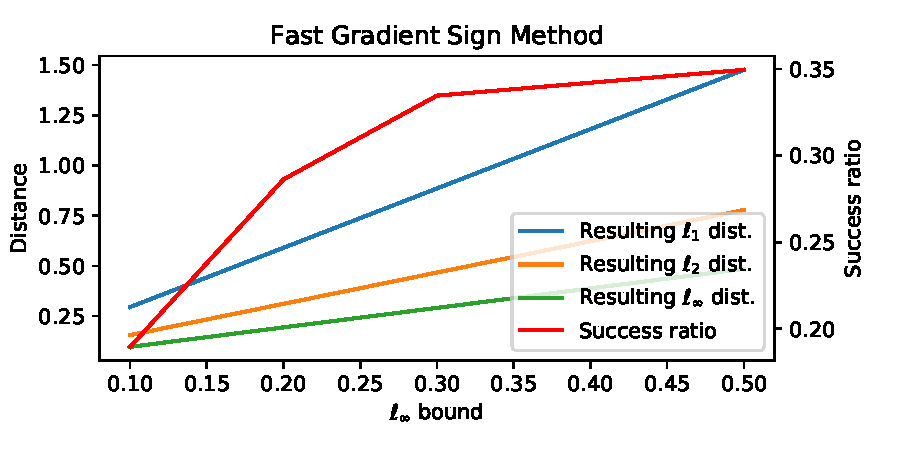
\includegraphics[width=0.49\textwidth]{adv_plots/fgsm.pdf}
%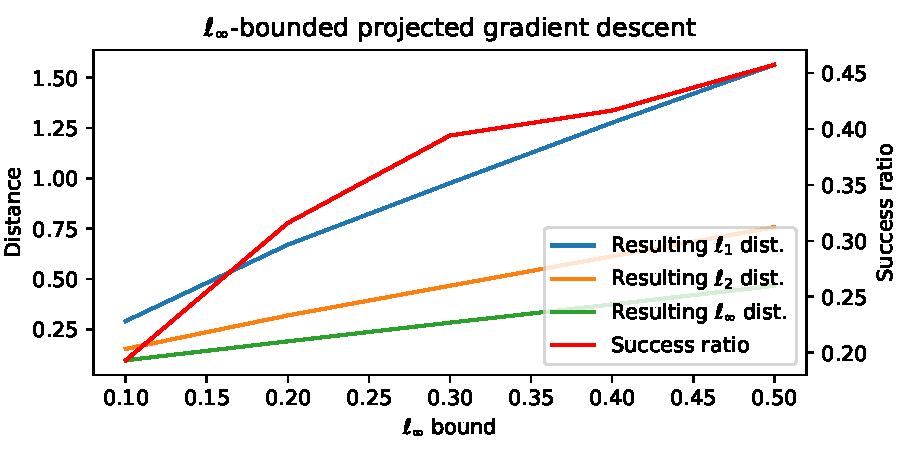
\includegraphics[width=0.49\textwidth]{adv_plots/l_inf_pgd.pdf}
%\caption{Performance of FSGM and $\ell_\infty$-bounded \gls{pgd} for different bounds.
%\todo{Max: Omit}}
%\label{fig:fgsm}
%\end{figure*}

%Finally, we investigated what adversarial flows look like and which features are manipulated to circumvent detection by the neural network.
%
%To this end, we generated adversarial flows with the \gls{cw} with $\ell_2$ distance and a tradeoff of 0.5. \autoref{adv_plots} depicts how the method manipulates flows for some exemplary attack categories. Depicted is the mean of both unmodified flows and adversarial flows  of samples of individual attack families considering both \gls{iat} and packet length.
%
%The plots show that primarily features at the beginning of flows are modified. It is remarkable that it seems most promising to modify single packets while leaving most of the flow unchanged. In other cases, however, like depicted for the infiltration attack at the bottom, adversarial flows assume a complex pattern to circumvent detection.

%\begin{figure*}[p]
%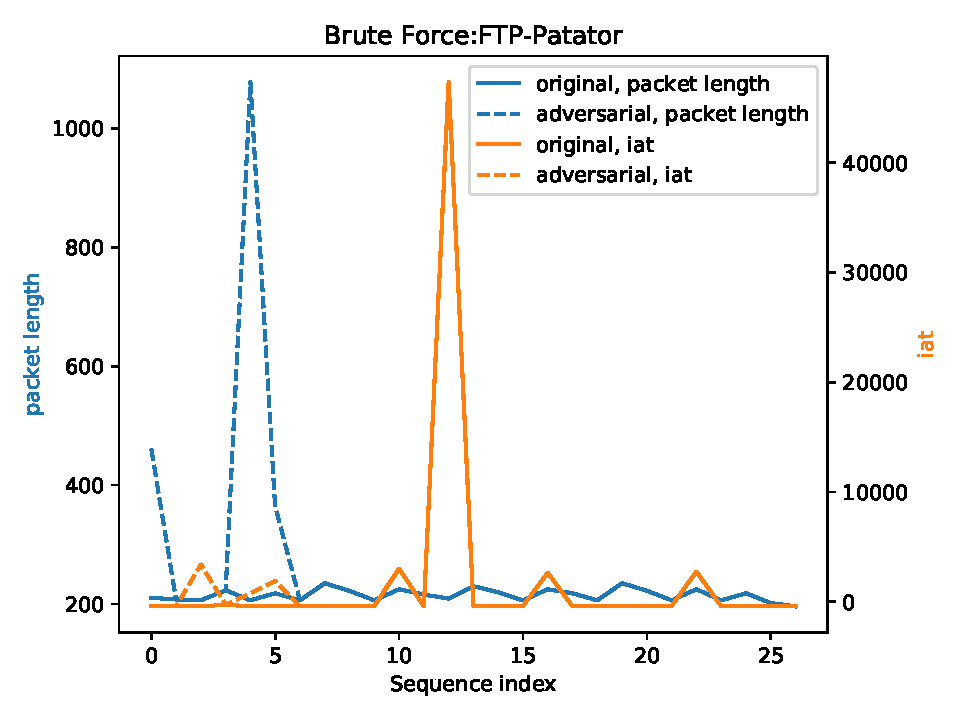
\includegraphics[width=0.48\textwidth]{../plots/plot_adv/1.pdf}
%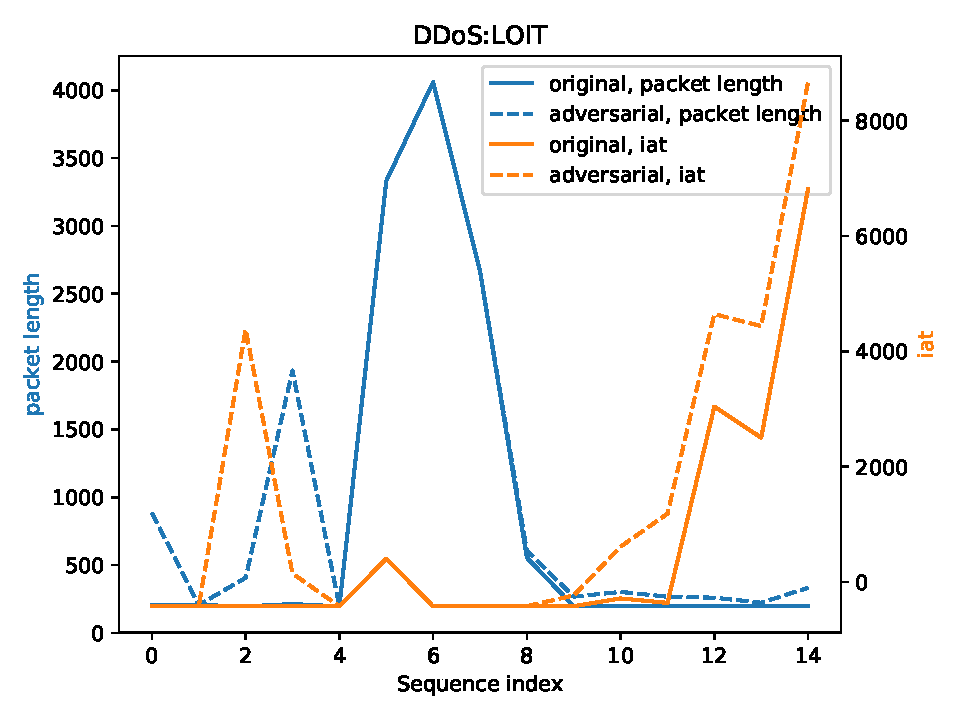
\includegraphics[width=0.48\textwidth]{../plots/plot_adv/2.pdf}
%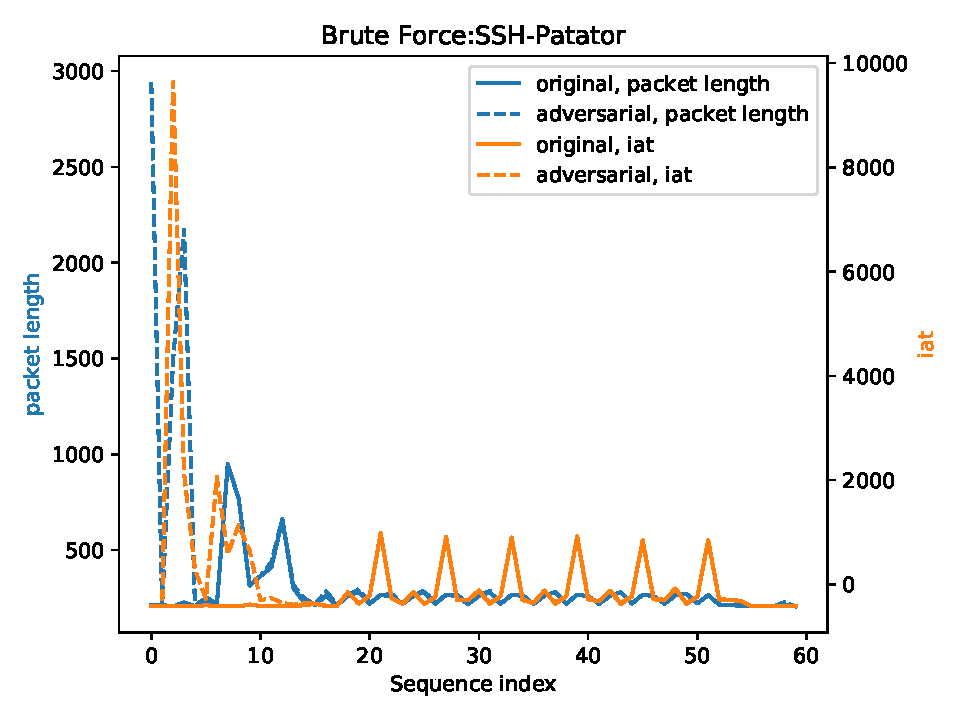
\includegraphics[width=0.48\textwidth]{../plots/plot_adv/3.pdf}
%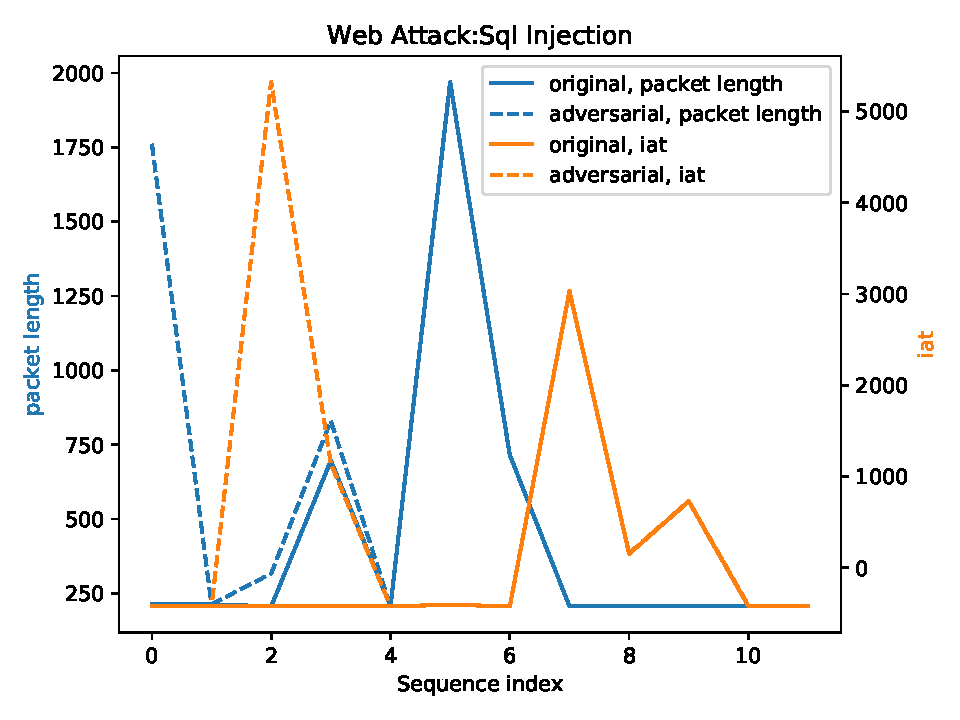
\includegraphics[width=0.48\textwidth]{../plots/plot_adv/4.pdf}
%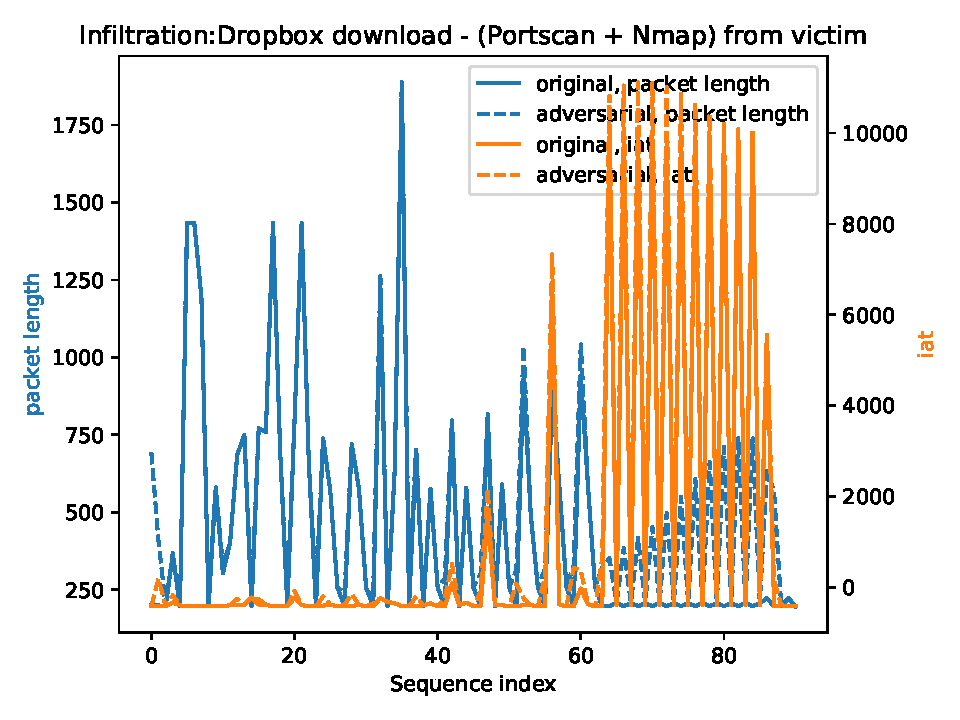
\includegraphics[width=0.48\textwidth]{../plots/plot_adv/5.pdf}
%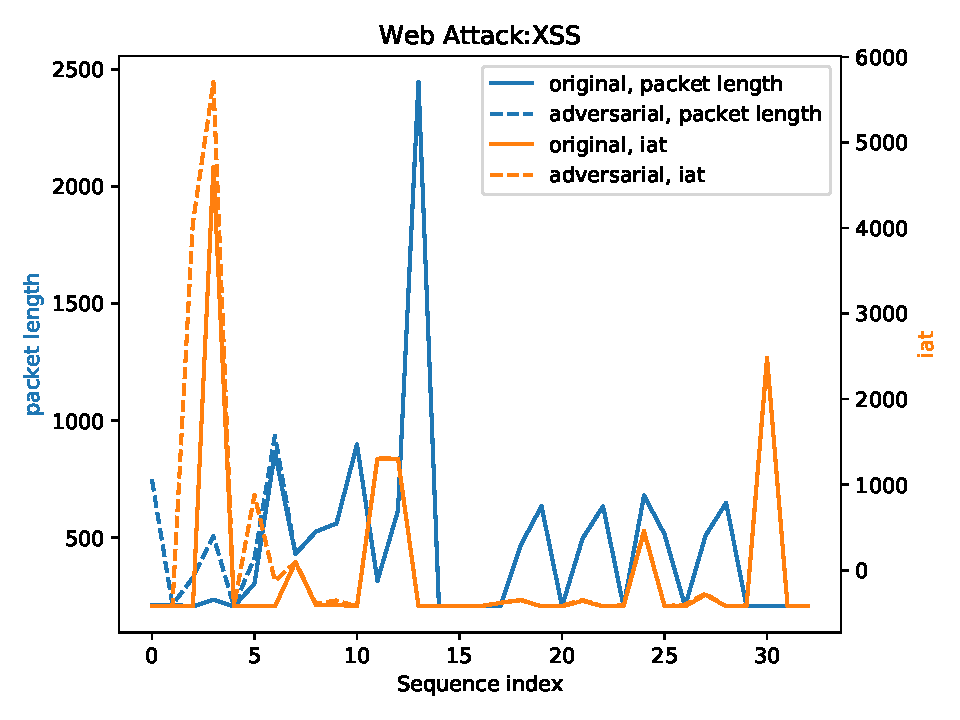
\includegraphics[width=0.48\textwidth]{../plots/plot_adv/6.pdf}
%\caption{Successful manipulations performed by the \gls{cw}. \todo{Max: Just keep one plot I'd say. Maximum two.}}
%\label{adv_plots}
%\end{figure*}

\section{Adversarial Robustness Metric}

As \autoref{fig:adv_per_family} and \autoref{tab:adv_accuracies} show, for most attack types, most samples can be modified by an adversary to be classified as benign by using \gls{cw}. High accuracy for a particular attack category does not imply that adversarial attacks are  likely to fail for these attacks. Thus we argue that beside the classical metrics such as accuracy, false positives etc., a new metric is needed, which quantifies how easily a classifier can be fooled. 

Such a method should be easy to compute and easy to interpret. We thus propose the \gls{ars}, which roughly works as follows: Use \gls{cw} with a small tradeoff to try to generate adversarial samples for an attack type. If more than half of the samples are now wrongly classified, stop. Otherwise increase the tradeoff of \gls{cw} and repeat. If after a predefined number of iterations -- e.g. 100 -- still not more than half of the samples are adversarial, also break. 

The result is a number of adversarial samples (more than half in the ideal case) and some that could not be made adversarial. For example, if in total, there are 100 samples, there might be 54 which could be made adversarial. Out of these 54, the 50 with the smallest distance to the original samples are taken. Of these samples, the distance of each adversarial sample to the original sample is taken and averaged over all 50 samples. The resulting average distance is the \gls{ars}. The larger it is the better since then an adversary needs to modify the samples more to make them adversarial. If not more then half of the samples could be made adversarial, our metric is undefined since then apparently it is not possible for an adversary conduct adversarial attacks on the majority of samples.

Setting the threshold for the \gls{ars} to 50\% is arbitrary, but
 reasonable as this way the \gls{ars} approximates the median of the distances of all samples and, additionally, marks the distance where an adversarial attack is more likely to be successful than unsuccessful.
%we think that it is reasonable since if an attacker can make the majority of samples adversarial, we think that its attack is ``successful''.

\todo{Insert results}

\section{Explaining Recurrent Neural Networks}
From a naive perspective, one might be tempted to reuse explainability methods for \glspl{rnn} by considering a flow the sum of its packet features.
We identify several difficulties which occur when trying to explain decisions made by \glspl{rnn}. 

\begin{itemize}[topsep=0pt,wide,labelwidth=!,labelindent=0pt]
\item
\textbf{Feature quantity.}
The number of features that is fed into an \gls{rnn} is found as the product of packet features with the total length of the flow. For long flows, the total number of inputs can therefore grow to a substantial size.

\item
\textbf{Variable sequence lengths.}
The length of different flows might differ tremendously. Hence, features which are important for the network's outcome for one flow might not even exist for other flows. Furthermore, the question arises how the distance between flows of different length can be computed.

\item
\textbf{Lack of a distance measure.}
However, even if we restricted the analysis to flows of a constant length, a flow is different from the plain concatenation of its packet features.
If we, for example, consider a classification problem as in this document, we expect that after a certain amount of time steps the classifier is able to perform the classification with a certain confidence. Arguably, features at the beginning of a flow are thus more important for the classifier. Giving feature differences at the end of a flow the same weight as differences at its beginning, therefore seems incorrect.

\item
\textbf{Multiple prediction outputs.}
Often an \gls{rnn} produces an output at each time step. When trying to apply explainability methods, hence, the question arises which output to base the methods on. The natural choice is to base the methods on the prediction output which occurs at the same time step as the feature under investigation. Not only does this approach require a substantially lower amount of computational resources compared to predictions occurring at a later time step, but we also expect the immediately occurring prediction outcome to exhibit a stronger correlation to the feature under investigation, compared to a prediction outcome occurring many time steps later.
However, due to the complex decision processes that can occur for deep neural networks, it is absolutely  uncertain if the network's final prediction is correctly depicted when following this approach.
\end{itemize}

Many explainability methods proposed recently are local and thus provide explanations for a particular data sample \cite{shapley_value_1953,lundberg_unified_2017,dhurandhar_model_2018,ribeiro_why_2016}. However, for the particular problem of network traffic, due to the high number of flows and the characteristics of data, analyzing individual samples is of low interest. Explainability methods presented in this paper therefore aim to understand a model by analyzing which features are important, at which time step they are important and which feature values lead to classification as attack.

% where does this come from :)
%\subfloat[Throughput of the fq \gls{qdisc}\label{fig:fqThroughput}
%]{
%\includegraphics[width=\columnwidth]{{{plots/throughput_1_fq_cubic_10_20_60_0.5_bw_1571240937211.pcap}}}
%}{}

\subsection{Feature Importance Metrics}
\begin{table}
\caption{Accuracy drop for:}
\label{tab:feat_importance}
\centering
\subfloat[Random replacement method\label{fig:featRandom}
]{
\begin{tabular}{l r}
\toprule
Feature & \hspace*{-4mm}Accuracy~drop \\ \midrule
Protocol & 0.207 \\
Packet Length & 0.165 \\
SYN Flag & 0.099 \\
ACK Flag & 0.084 \\
Direction & 0.073 \\
Destination port & 0.071 \\
Source port & 0.060 \\
RST Flag & 0.057 \\
PSH Flag & 0.056 \\
Interarrival time & 0.024 \\
FIN Flag & 0.012 \\
URG Flag & 0 \\
ECE Flag & 0 \\
CWR Flag & 0 \\
NS Flag & 0 \\
\bottomrule
\end{tabular}
}{}
\subfloat[Feature dropout\label{fig:featDropout}
]{
\begin{tabular}{l r}
\toprule
Feature & \hspace*{-4mm}Accuracy~drop \\ \midrule
Destination port & 0.025 \\
Source port & 0.003 \\
RST Flag & 0.001 \\
ACK Flag & 0.001 \\
Protocol & 0.001 \\
Packet Length & 0.001 \\
Direction & 0.001 \\
SYN Flag & 0 \\
Interarrival time & 0 \\
FIN Flag & 0 \\
ECE Flag & 0 \\
URG Flag & 0 \\
CWR Flag & 0 \\
NS Flag & 0 \\
PSH Flag & 0 \\
\bottomrule
\end{tabular}
}{}
\end{table}
As a first step to understanding the neural network's decisions, we  estimate how important individual features are for the model's predictions.
When investigating an \gls{ml} classifier, it is natural to ask which inputs have a large influence on the classifier's prediction. We feel the need to distinguish metrics for this purpose based on their main aim:

A large amount of research has been spent on finding \emph{feature importance} metrics, which allow the selection  of high-importance features, providing a reasonably good classification performance while resulting in a more light-weight classifier.

On the other hand, both adversarial machine learning and explainable machine learning bring up the question to what extent individual features are able to change the prediction outcome. While being seemingly similar at first sight, traditional feature importance can yield markedly wrong results for this case.  To distinguish, we propose the term \emph{feature sensitivity} for such metrics.

To analyze features for our network, we use the following approaches.

\subsubsection{Neural Network Weights}
In previous works~\cite{olden_accurate_2004}, a simple method for determining feature importance in neural networks, has been summing up neural network weights leading from a certain input to the prediction outcome. The weights method can be considered for both feature importance and feature sensitivity, however, clearly, especially in the case of complex network architectures, this method is likely to provide wrong results. Hence, we provide results for the weights method mainly for comparison. Note that an LSTM cell alone has four weights leading from one input to an output. 

\subsubsection{Input Perturbation}

 The most commonly used techniques for feature importance which are used by practitioners for \glspl{rnn} \cite{stackexchange_cross_validated_neural_2019} and \gls{dl} \cite{molnar_interpretable_2019,stackexchange_cross_validated_feature_2016} in general are based on adding noise to a particular feature and then evaluating the drop in accuracy that occurs. We argue that it is hard to find out the ``correct'' intensity of noise to add, we slightly vary the proposed approach: We do not add noise drawn from a probability distribution but instead sample the value for a feature from the distribution of all values of this feature. This makes the method non-parametric since the distribution of the noise does not need to be chosen. We ensured that features which stay constant for a flow, i.e. source port, destination port and protocol, also stay constant throughout the whole flow when randomizing the feature.


\subsubsection{Feature Dropout}
While the method of adding noise to features/randomizing them is convenient since it is easy to implement and understand, we argue that it has some shortcomings: 
The \gls{rnn} was never trained for dealing with ``garbage'' values that the noise/randomization methods create. For example, completely unrealistic feature combinations could occur that were never observed during training. Furthermore, sequences of features could occur that cannot occur in reality. 
 
%We think that the ``ideal'' feature importance method for our scenario are Shapley values \cite{shapley_value_1953}: To analyze feature importance with them, the feature under investigation is completely omitted from the dataset and a model is trained without it. The resulting accuracy is then compared to the baseline accuracy with all features. The effort required to do this is high both in terms of storage space as well as training time since for $n$ features $n$ models need to be separately trained and stored. While this seems tractable, when also analyzing the feature importance of combinations of features, the number of models required becomes even larger: Out of $n$ features, $2^n$ unique subsets can be chosen, meaning that the computational demand rises exponentially. 

We thus develop a more sound method compared to input perturbation called \textit{feature dropout}: When training a model, for each sample, we leave out each feature with a certain probability by setting it to zero. On average, one feature gets zeroed out but it is also possible that none or more than one are left out. This procedure is equivalent to using dropout \cite{srivastava_dropout:_2014} with probability $\frac{1}{n}$ before the first layer. An important implementation detail here is that for each feature we add another input which is 1 if the feature is suppressed and 0 otherwise. This is necessary so that the neural network can distinguish between a feature missing and a feature genuinely being zero. The overall outcome is a classifier being able to deal with missing features. As it can also happen that several features are left out for a sample, our method can also be used to analyze the effect of multiple features missing and can thus show possibly correlated features. The results in Table~\ref{fig:featDropout} show that, unlike the randomization feature importance method, the feature dropout method does not vastly overestimate features' importance. With feature dropout, it becomes apparent that there are very few features that actually contain unique information and that affect accuracy when left out: the destination port and the source port. A model trained with feature dropout typically yields slightly lower accuracy than a regularly trained model, even if no features are left out (flow accuracy of 0.9943 vs.~0.9965. We thus recommend training two models: One regular one and one with feature dropout to use for the feature importance. Another method that uses dropout for feature importance is \cite{chang_dropout_2017}, which, however, applies a technique called \textit{Variational Dropout} to learn the optimal dropout rate for each feature. It tries to leave out as many features as possible and at the same time keep accuracy high. Thus important features are going to be left out less often and one can then extract the dropout probabilities for each feature and assess their significance based on them. Feature dropout can also be used as a building block for computing the accuracy of datapoints with missing features that is necessary to compute Shapley values \cite{shapley_value_1953} or KernelSHAP \cite{lundberg_unified_2017}.

Feature dropout also allows us to find correlated features or -- more general -- features that contain common information: 

\begin{equation}
\text{score} = \frac{\text{acc}_\text{base}-\text{acc}_\text{-both\_features}}{\left(\text{acc}_\text{base}-\text{acc}_\text{-feature\_1}\right) + \left(\text{acc}_\text{base}-\text{acc}_\text{-feature\_2}\right)}
\end{equation}
With $\text{acc}_\text{base}$ we denote the average accuracy of the classifier with all features included, with $\text{acc}_\text{-feature\_i}$ the average accuracy if feature $i$ is omitted and with $\text{acc}_\text{-both\_features}$ the average accuracy if both features are omitted. The higher the resulting number, the larger the information that both features share. If the score is one, this means that both features contain no joint information. For example, the score between RST and the protocol identifier is 8.5; the highest of all pairs of features. While this may seem unintuitive at the first glance, it likely stems from the fact that if the protocol identifier (\gls{tcp} or UDP) is missing, then if RST is 1 at some point of the flow, the flow has to be \gls{tcp}.

\subsubsection{Mutual Information}
\begin{figure}
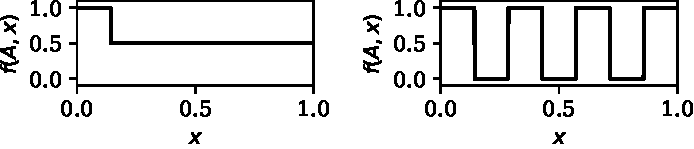
\includegraphics[width=\columnwidth]{../plots/mutinfo_example.pdf}
\caption{Two distributions yielding an identical accuracy drop.}
\label{fig:mutinfo_example}
\end{figure}
Input Perturbation has some shortcomings when considering feature sensitivity. Assuming that the test dataset is representative for production use, for feature importance it is reasonable to equate the distribution of the perturbed feature with the feature distribution. On the other hand, when evaluating feature sensitivity, e.g. for analyzing potential for adversarial samples, the attacker is not limited by this distribution and frequently is able to choose arbitrary values in the feature space.

Furthermore, let $f(A,x)$  denote the joint probability
%\todo{Max: Ist joint probability nicht immer wenn man mehrere Ereignisse hat? Ich hätte hier probability density function geschrieben...}
%AH. changed notation and wording
for classification as attack and a feature value $x$. Accuracy then is $\int f(A,x) dx$ for attacks and $1-\int f(A,x) dx$ for benign traffic.
\autoref{fig:mutinfo_example} shows two different distributions
yielding the same accuracy, but clearly the right-side distribution has a larger influence on the prediction, as in the right-side case the prediction deterministically depends on the feature value.
To capture such dependencies, we propose to use mutual information instead of accuracy drop to determine feature sensitivity.
Mutual Information between two random variables $X,Y$ is defined as 
\begin{equation}
I_{X,Y} = \mathbb E \left\{ \log\left(\frac{f_{X,Y}(x,y)}{f_X(x)f_Y(y)}\right) \right\},
\end{equation}
with $f_X(x), f_Y(y)$ and $f_{X,Y}(x,y)$ denoting the distribution of $X,Y$ and their joint distribution, respectively. To obtain feature sensitivity, we compute mutual information between an input variable and the prediction output for one flow at one particular time step, and average over the result for the test dataset.

\subsubsection{Results}
\begin{figure*}
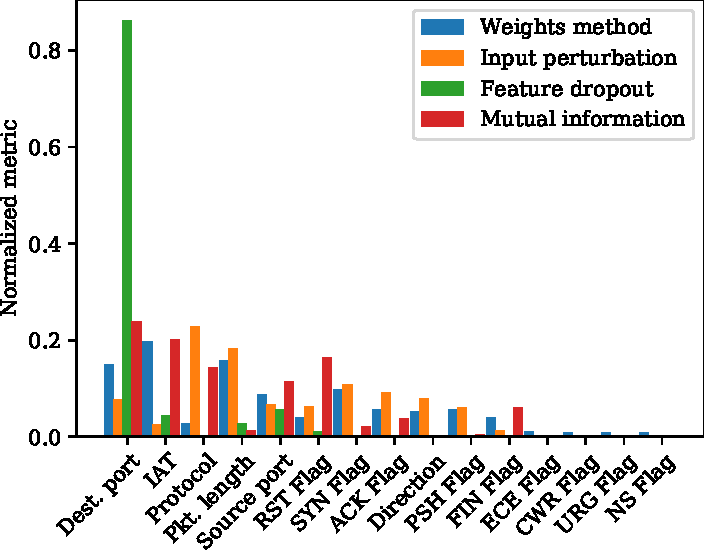
\includegraphics[width=.49\textwidth]{../plots/importance/feat_imp_flow_2017.pdf}\hspace{.02\textwidth}
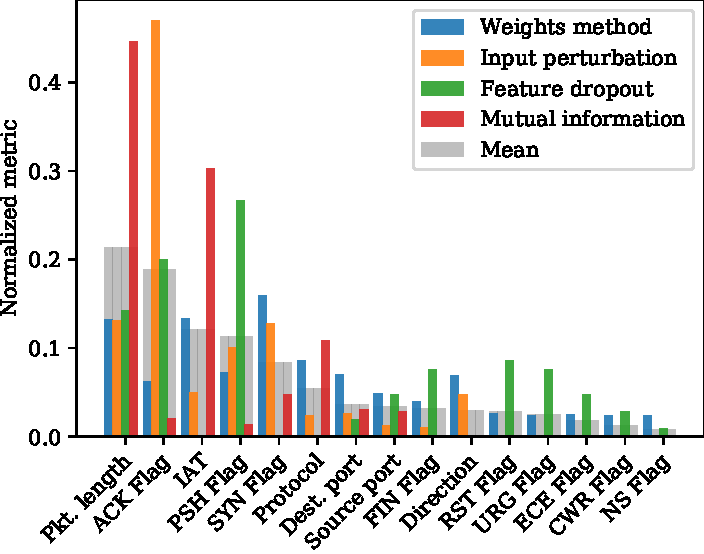
\includegraphics[width=.49\textwidth]{../plots/importance/feat_imp_flow_2015.pdf}
\caption{Feature importance metrics considering the final flow prediction for CIC-IDS-2017 (left side) and UNSW-NB15 (right side).}
\label{fig:feat_imp}
\end{figure*}
Table~\ref{fig:featRandom} and \autoref{fig:feat_imp} show the results, which match to a large extent with domain-specific expectations for classifying network flows.
In particular, rarely used \gls{tcp} flags like NS or URG are unimportant for the classifier. On the other hand, destination port and protocol are essential for characterizing flows by hinting at the type of traffic. \gls{iat} and packet length are important for estimating the amount of transferred information and several flags hint at certain attacks like \gls{dos} attacks.

The weights method is able to reveal features with a very low importance to a certain degree, but disagrees with the other methods to a large extent. Less anticipated, however, also input perturbation does not exhibit a considerable correlation with feature dropout. Considering its functioning, feature dropout is the most reliable method for evaluating importance for removing features. It is remarkable that none of the other methods is able to depict the distinct peak of importance for the destination port. 

It is not surprising that mutual information disagrees with feature dropout, since both their aim and their functioning are substantially different. For example, mutual information shows that the protocol field can have a substantial impact on the classification even though an identical accuracy can be achieved when omitting it.

% In particular, the most important features turn out to be the used protocol, packet length and the SYN TCP flag. While the first two features are essential for characterizing flows, a high number of packets with set SYN flag is an important characteristic for port scanning or certain DoS attacks. Also the fact that most of TCP flags do not play an important role in our dataset was expected. It is interesting to note, however, that the interarrival time of packets does not play a crucial role for the detection of attacks. 

Note that metrics for UNSW-NB15 differ substantially from CIC-IDS2017. However, due to the large number of different network attacks and network configurations, it is easily possible that different features are relevant for both datasets. We consider the question of model transferability of substantial importance for the presented application, but out of scope for the present research.

\subsection{Explainability Plots}
Knowing which features to investigate, it is important to analyze which feature values lead to classification as attack.
During flow extraction we used a usual 5-tuple flow key, which distinguishes flows based on the protocol they use and their source and destination port and IP address. Hence, these features are constant for all packets in one flow, which allows us to use explainability methods which have been proposed for non-recurrent classification methods.

In particular,  in literature the use of Partial Dependency Plots (\gls{pdp}) is proposed~\cite{friedman_greedy_2001}. To inspect attack types in detail, in this research we experiment with a modified definition of the \gls{pdp}. If $\boldsymbol X \in \mathbb R ^n$ denotes a random vector drawn from feature space, $f(X) \in [0,1]$ denotes the neural network's prediction and $c$ the attack class, the \gls{pdp} for feature $i$ can be defined as
% \begin{equation} \label{eq:pdp}
% \text{\gls{pdp}}_i(y) = \mathbb E_{\boldsymbol X}\left(f(X_1,\ldots,X_{i-1},y,X_{i+1},\ldots X_n)\right)
% \end{equation}

% To inspect attack types in detail, in this research we experiment with a modified definition of the \gls{pdp}  (with C being the attack classes):
\begin{equation} \label{eq:pdp_conditional}
\text{\gls{pdp}}_{c,i}(y) = \mathbb E_{\boldsymbol X | C = c} \left(f \left( X_1,\ldots,X_{i-1},y,X_{i+1},\ldots X_n \right) \right)
\end{equation}
%
%\begin{figure*}
%\includegraphics[width=0.48\textwidth]{{"../plots/plot_pdp/flows_full_no_ttl_pdp_outcomes_0_3.pickle_8_DoS - DDoS-Heartbleed"}.pdf}
%\includegraphics[width=0.48\textwidth]{{"../plots/plot_pdp/flows_full_no_ttl_pdp_outcomes_0_3.pickle_10_Normal"}.pdf}
%
%\caption{Examples of conditional PD plots for source and destination port. We only analyze these features with the \gls{pdp} since it is not straightforward to define the \gls{pdp} for features that can vary for each packet in a flow. The y-axis shows the probability for malicious traffic.}
%\todo{Max: Remove these? Not really interesting or related to the rest of the paper. Refer to other paper where we talk about this already.}
%\label{fig:pdp}
%\end{figure*}
%
In this variant of the \gls{pdp} that we call conditional \gls{pdp}, we don't take the whole dataset for the computation for the \gls{pdp} but only a subset that belongs to a certain class. Specifically, we take each attack class and compute the \gls{pdp} only over samples of this attack class. The results (omitted for brevity) show that for some attack classes the port numbers play an important role. When looking at the class of normal traffic (non-attack traffic) it becomes apparent that traffic destined to a high source port is generally indicative of an attack. We argue that this is because most services that regular users use have low port numbers. A known issue about \glspl{pdp} in general is that dependencies of the feature under investigation and the remaining variables are not considered, hence potentially querying the neural network for feature combinations which cannot possibly occur. For a certain value of the $i$th feature, the whole dataset is used for averaging the neural network's outcome. 

%For this reason, Accumulated Local Effects (ALE) plots have been proposed in literature. The basic idea for ALE is that instead of using all samples, only the closest samples are used for assessing the effects of one feature. ALE plots therefore inherently require a distance measure for finding the closest samples, which, as revealed in the above discussion, in our case is not possible in a straight-forward manner.

\subsection{Plots for Sequences}

As apparent from the above discussion, trying to explain how packet features influence the model's predictions, poses various difficulties. As a first step to explaining our model's predictions, we investigate how important features at different time steps are for the model's decisions. Intuitively, features at the beginning of a flow should be the most important while the model's predictions should not vary significantly anymore, as soon as the model has come to a decision.

\begin{figure}
%\includegraphics[width=0.48\textwidth]{{"../plots/plot/flows_pred_plots2_outcomes_0_3.pickle_5_DoS - DDoS-DoS Hulk"}.pdf}
\includegraphics[width=\columnwidth]{{"../plots/plot/flows_pred_plots2_outcomes_0_3.pickle_6_DoS - DDoS-DoS Slowhttptest"}.pdf}
% \includegraphics[width=0.48\textwidth]{{"../plots/plot/flows_full_no_ttl_pred_plots_outcomes_0_3.pickle_14_Web Attack-XSS"}.pdf}
% \includegraphics[width=0.48\textwidth]{{"../plots/plot/flows_full_no_ttl_pred_plots_outcomes_0_3.pickle_11_PortScan-PortScan - Firewall off"}.pdf}

\caption{Median confidence per time step and first and third quartiles. For the majority of attacks types, confidence increases in the first few steps and then stays almost constant at 1.}
\label{fig:confidence}
\end{figure}

To determine if this hypothesis is correct, we plot the attack confidence of the classifier for each time step for each attack class. At each time step we average over all flows and also show the first and third quartiles. \autoref{fig:confidence} shows that this hypothesis is correct for most attack classes. At the first couple of packets the confidence for maliciousness is not very high yet but towards the end of the flow it reaches values close to 1 and stays there.

\begin{figure}
%\includegraphics[width=0.48\textwidth]{{"../plots/plot2_adv/flows_pred_plots2_outcomes_flows_adv_1.0_notBidirectional_outcomes_0_3.pickle_0_3.pickle_0_Botnet-ARES"}.pdf}
\includegraphics[width=\columnwidth]{{"../plots/plot2_adv/flows_pred_plots2_outcomes_flows_adv_1.0_notBidirectional_outcomes_0_3.pickle_0_3.pickle_7_DoS - DDoS-DoS slowloris"}.pdf}
%\includegraphics[width=0.48\textwidth]{{"../plots/plot2_adv/flows_pred_plots2_outcomes_flows_adv_1.0_notBidirectional_outcomes_0_3.pickle_0_3.pickle_11_PortScan-PortScan - Firewall off"}.pdf}
%\includegraphics[width=0.48\textwidth]{{"../plots/plot2_adv/flows_pred_plots2_outcomes_flows_adv_1.0_notBidirectional_outcomes_0_3.pickle_0_3.pickle_1_Brute Force-FTP-Patator"}.pdf}

\caption{Exemplary PD plot and adversarial flows for the DoS Slowloris attack in CIC-IDS-2017. The solid line shows the mean value of the feature for all flows of the attack type. The shaded region shows the change in confidence that occurs when the feature is varied. \todo{IAT plot is wrong: There shouldn't be step 0.}}
\label{fig:pred_plots2}
\end{figure}

Next, we want to investigate if our classifier just memorized its inputs. The most interesting packet features that can be used to visualize this in our use case are the \gls{iat} between packets in a flows and the packet length. To depict how the model comes to a decision, we determined the total minimum and maximum for these features that ever occur for all flows. For a given flow $X$ we then varied feature values at each time step between minimum and maximum and plot how the confidence changes when the feature varies (\autoref{fig:pred_plots2}) depict the averaged predictions for different attack families. It seems clear that the classifier didn't just memorize the inputs but actually learned them since there is always a smooth decrease of confidence if we change the feature values. Instead, when memorizing, we would expect a sharp decline of confidence to occur. Another interesting observation is that after the first couple of packets the classifier is certain about its decision and changing features doesn't change its confidence any longer. This allows the conclusion that if an attacker is able to change the first few packets, she could possibly change the decision of the classifier. We will further investigate this question in \autoref{sec:adv}.

\begin{figure}
%AH. I think the 'Firewall off' plot is not a good example as it shows only 4 packets
\includegraphics[width=\columnwidth]{{"../plots/plot_features/flows_pred_plots2_outcomes_0_3.pickle_2_Brute Force-SSH-Patator"}.pdf}
%\includegraphics[width=0.48\textwidth]{{"../plots/plot_features/flows_full_no_ttl_pred_plots2_outcomes_0_3.pickle_6_DoS - DDoS-DoS Slowhttptest"}.pdf}
%\includegraphics[width=\columnwidth]{{"../plots/plot_features/flows_full_no_ttl_pred_plots2_outcomes_0_3.pickle_11_PortScan-PortScan - Firewall off"}.pdf}
%\includegraphics[width=0.48\textwidth]{{"../plots/plot_features/flows_full_no_ttl_pred_plots2_outcomes_0_3.pickle_7_DoS - DDoS-DoS slowloris"}.pdf}

\caption{\gls{iat} and packet length for SSH brute-force attacks in CIC-IDS-2017.}% The solid line shows the median value of the feature for all flows of a specific attack type. The shaded region are the first and third quartile.} % think legend is enough for unterstanding
\label{fig:plot_features}
\end{figure}

Looking at the plots of the features that vary over time (\autoref{fig:plot_features}) we see that certain attack types have a characteristic pattern in which they send packets by which they are easily recognizable. We want to determine how the pattern of packet sizes and \glspl{iat} is significant for the classification. \autoref{fig:plot_features} clearly shows that some attack types have very characteristic patterns of packet sizes and \glspl{iat}.

\section{Defences}
We now propose two approaches to increase robustness of the \gls{rnn} against adversarial attacks.
\subsection{Reducing features}
The most obvious defence, which is only possible because of the nature of the dataset, is to simply leave out features which the attacker can manipulate. For this, we try two different approaches:
\begin{itemize}[topsep=0pt,wide,labelwidth=!,labelindent=0pt]
\item Leaving out all manipulable features: packet size and \gls{iat}
\item Leaving out manipulable features when the attacker can manipulate them: only in the direction from the attacker to the victim (This, however does not prevent adversarial samples for botnets, for which both sides are malicious)
\end{itemize}

Both approaches lead to complete resistance to adversarial samples (as we left out all manipulable features), except for botnets, which can still operate when only leaving out manipulable features in one direction. The results show that -- surprisingly -- there is only a small difference in classification performance when only computing the accuracy for the last packet of each flow (flow accuracy): Flow accuracy stays over 99.93\%. However, packet accuracy is only 98\% when leaving out the features in one direction and 96.7\% when leaving them out in both directions, Thus, apparently the \gls{iat} and packet size are especially important for determining whether a flow is malicious in the first packets of a flow.

\subsection{Adversarial training}
As alternative to omitting manipulable features, we attempted to make the classifier more robust against adversarial samples by augmenting the training set by adversarial flows generated using  \gls{cw}, labeled as additional attacks.

For this purpose, we added one adversarial sample per attack sample to the training set. Since \gls{cw} is deterministic, this is the maximum number of adversarial samples possible. With this training set we then alternated retraining of the neural network and optimization of the adversarial samples using gradient descent.

A question which occurs in this process, is how many CPU cycles to spend on network training and adversarial sample optimization. As a natural approach, we decided to use as many backpropagation steps for neural network training as we use for adversarial sample optimization.  For each adversarial sample optimization step, we performed 10 iterations of gradient descent. Hence, all adversarial samples were optimized each 10 epochs of neural network training.

\autoref{fig:avdistance} shows the \gls{ars} throughout the adversarial training procedure for several attack categories and clearly indicates that adversarial training is effective, as the distance gradually increases. Hence, an attacker would have to modify attack samples more and more, eventually rendering the attack unpractical.

%However, the figure also shows that an increase of distance can only be achieved after a considerable amount of training. It is, hence, questionable if the gained increase in robustness is enough for reliable attack detection.



\begin{figure}
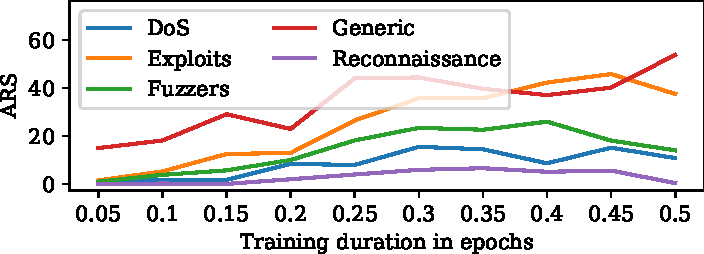
\includegraphics[width=\columnwidth]{../plots/ars/ars_15.pdf}
\caption{\gls{ars} during adversarial training for UNSW-NB15.}
\label{fig:avdistance}
\end{figure}

For both datasets, after a small number of epochs, it was no longer possible to create a significant number of adversarial samples for most attack categories. For the datasets we considered, adversarial training left classification performance unaffected.
%\todo{Max: Insert results that show that accuracy on normal data is still ok after adversarial training.}

\autoref{tab:adv_training_performance} depicts classification on non-adversarial data after 50 epochs of adversarial training. Accuracy is essentially identical to results presented in \autoref{tab:performance_results}. Due to the higher proportion of attack samples in training data, we note, however, that recall increased at the expense of a slightly lower precision. 


\begin{table}
% Evaluated using
% ./python learn.py --dataroot flows.pickle --net runs/Oct26_00-03-50_gpu/lstm_module_1284.pth --function test --batchSize 512
% ./python learn.py --dataroot flows15.pickle --net runs/Oct28_15-41-46_gpu/lstm_module_997.pth --function test --batchSize 512
% on Dec. 4th
\caption{Detection performance after adversarial training.} \label{tab:adv_training_performance}
\todo{Probably no space for table}
\centering
\begin{tabular}{l r r r r} \toprule
& \multicolumn{2}{c}{CIC-IDS-17} & \multicolumn{2}{c}{UNSW-NB-15} \\
	&	Packet	&	Flow	&	Packet	&	Flow	\\	\midrule
Accuracy	&	0.991	&	0.997	&	0.994	&	0.981	\\
Precision	&	0.971	&	0.996	&	0.761	&	0.704	\\
Recall	&	0.979	&	0.992	&	0.970	&	0.824	\\
F1	&	0.975	&	0.994	&	0.853	&	0.759	\\
Youden	&	0.973	&	0.991	&	0.965	&	0.811	\\


\bottomrule
\end{tabular}
\end{table}

% AH. guess this is no longer true
%However, against our expectations, this approach did not lead to satisfactory results in the sense that the network would learn to classify adversarial samples as attacks. In fact, classification accuracy stayed about constant during the training of the network.

%A possible explanation for this observation might be that the adversarial samples assumed too much the shape of normal flows, so that the network could not reliable tell them apart.

%\begin{table*}
%\caption{Comparing performance with all features, only safe features (\gls{iat} and packet size removed) and safe features in one direction (\gls{iat} and packet size removed for packets coming from source). \textit{packets} means that we consider the neural network output of all packets of the flow while \textit{flows} means that we only consider the last packet. At the last packet the classifier is usually already a lot more confident than at the first packets of a flow and thus metrics are always better in this case. \todo{Max: Is this that interesting? Remove tables and inline the most interesting results?}}  \label{tab:performance_results_no_manipulable}
%\newcommand{\cmidrulespace}{6pt}
%\centering
%\begin{tabular}{l l l l l l l} \toprule
%& \multicolumn{2}{l}{all} & \multicolumn{2}{l}{safe features} & \multicolumn{2}{l}{safe features one direction} \\
%\cmidrule(r){2-3} \cmidrule(lr){4-5} \cmidrule(l){6-7}
%& packets & flows & packets & flows & packets & flows \\
%\midrule
%Accuracy & 0.9857054 & 0.99472587 & 0.96678023 & 0.99337596 & 0.98056073 & 0.99353386 \\
%Precision & 0.94963342 & 0.9894422 & 0.87175275 & 0.98798596 & 0.91359787 & 0.98994595 \\
%Recall & 0.96735895 & 0.98972051 & 0.94374958 & 0.98581328 & 0.97836672 & 0.9844478 \\
%F1 & 0.95841423 & 0.98958134 & 0.90632359 & 0.98689842 & 0.94487366 & 0.98718922 \\
%Youden & 0.95682951 & 0.98614231 & 0.91525628 & 0.98175163 & 0.95937772 & 0.9810602 \\
%\bottomrule
%\end{tabular}
%\end{table*}


\section{Conclusion}

We have implemented a recurrent classifier based on LSTMs to detect network attacks, %While attack detection performance is not necessarily better than that of non-recurrent approaches,
which can already detect attacks before they are over. Furthermore, the recurrent approach allows us to inspect the influence of single packets on the detection performance and shows which packets are \textit{characteristic} for attacks. 
Even though the interpretation of \glspl{rnn} poses several difficulties, we have demonstrated methods for gaining insights into the model's functioning.

We showed that even though our use case is very different from computer vision, adversarial samples can be found efficiently, even if only ostensibly unimportant features can be modified. We introduced the \gls{ars} as a new way to quantify the adversarial threat.
Deploying an adversarial training procedure, we could significantly reduce the adversarial threat.

\section*{Acknowledgements}
The Titan Xp used for this research was donated by the NVIDIA Corporation.


\renewcommand*{\bibfont}{\small}
\bibliographystyle{ieeetr}
\bibliography{bibliography}


\end{document}
\endinput
%%
%% End of file `sample-sigconf.tex'.
